\subsubsection{Defining Surface Energy}\label{define-surf-energy}
%TODO: Rewrite entire section in your own words in order to not copyright the author below. 
%\textbf{Interface Science and Composites (Chapter 3: Solid-Liquid Interface), by Soo-Jin Park and Min-Kang Seo\cite{Park2011a}}


Thermodynamically, the physical origin of the surface free energy is the excess Gibbs free energy of matter at the interface. Atoms or molecules exposed at an interface are surrounded by fewer neighbors, such as solid, liquid, and gas phases, resulting in an anisotropic distribution of these neighbors, which is the characteristic of a surface. Interaction energy must be shared between phases with the neighboring molecules. Hence, the surface free energy, $\gamma$, represents the rate of change of the Gibbs free energy of the system with respect to the area, $A$, at a constant pressure and temperature\cite{Chattoraj2012}:
\begin{equation}\label{SFE}
	\gamma = \left(\frac{\partial G}{\partial A}\right)_{T,P}
\end{equation}
In principle, Equation \ref{SFE} can be used to calculate the surface tension of a condensed phase held together by the long-range forces. 

The interaction of a liquid with a solid is characterized by the term "wetting." Wetting can be understood as the spreading of a liquid over a solid surface, the penetration of a liquid into porous materials, or the displacement of one liquid by another. This phenomenon can help to characterize a surface, and to determine the interaction between a solid and a liquid. 

One way to quantify a liquid's surface wetting characteristics is to measure the contact angle of a drop of liquid placed on the surface of an object. The contact angle formed by the solid-liquid and liquid-vapor interfaces are measured from the side of the liquid. Liquids wet surfaces when the contact angle is less than 90\degree. For a penetrant material to be effective, the contact angle should be as small as possible. In fact, the contact angle for most liquid penetrants approach 0\degree. 

The wetting ability of a liquid is a function of the surface energy of the solid-vapor interface, the liquid-gas interface, and the solid-liquid interface. The surface energy across an interface or the surface tension at the interface is a measure of the energy required to form the unit area of a new surface at the interface. The intermolecular bonds, or cohesive forces, between the molecules of a liquid cause surface tension. When the liquid encounters another substance, there is usually an attraction between the two materials. The adhesive forces between the liquid and the second substance will compete against the cohesive forces of the liquid.  Liquids with strong cohesive bonds and weaker adhesive forces will tend to bead-up or form a droplet when in contact with another material. Liquids with relatively weak cohesive bonds and a strong attraction to another material, or the desire to create adhesive bonds, will tend to spread over the material, such is the case with water droplets on high-surface energy metal substrates.

Depending on the thermodynamic state or the hydrodynamic status of the liquid drop in which the contact angle is measured, two types of contact angels can be defined. If the contact angle is measured when either the liquid drop contines to spread or when its thermodynamic state conditions continue to change, the measured contact angle is termed the dynamic contact angle. However, if the contact angle is measured under conditions in which the liquid drop is stationary and the surrounding conditions in which the liquid drop is stationary and the surrounding conditions are in the steady state, the measured contact angle is known as the static/equilibrium contact angle. The contact angle technique is chosen for studies of the wettability phenomena owing to its simplicity. 

The solid-liquid interface plays a fundamental role in diverse fields and helps with an understanding of physical phenomena and structural knowledge of the interface at the atomic scale. Fields of interest include catalysis, lubrication, electrochemistry, colloidal systems, biological reactions, and, most relevantly, crystal growth. Therefore, unravelling the atomic structure at the solid-liquid interface is one of the major challenges. 

Contact angle measurements, as described by Thomas Young in 1805, remain the most accurate method for determining the interaction energy between a liquid (L) and a solid (S) in a condensed state at the minimum equilibrium distance of S and L. This is defined geometrically as the angle formed by a liquid at the three-phase boundary, where vapor, liquid, and solid intersect. It measures the result of liquid cohesion energy, in the guise of $\gamma_{L}$ and the energy of adhesion between a liquid and solid. Young described the equilibrium contact angle at the three-phase boundary in terms of the vectorial sum, as shown in Figure \ref{fig:ca-vector}, resulting in an equilibrium force balance. The famous Young's equation is derived from the Gibbs free energy at equilibrium, as seen from the result of Equation \ref{youngs-eqn}. 

\begin{figure}
	\centering
	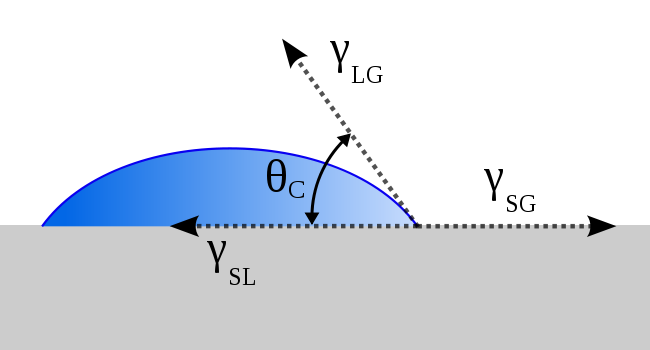
\includegraphics[width=0.7\textwidth]{Contact_angle}
	\caption{This illustration shows a vector representation of the interfacial tensions involved in a solid-liquid-gas contact angle experiment. [Image available in public domain: wikimedia.org]}
	\label{fig:ca-vector}
\end{figure}

%\begin{tcolorbox}
Derivation of Young's Equation\\
Assuming an ideally flat surface
\begin{equation} \label{dropvol}
V_{drop} = \frac{\pi R^{3}}{3} (1-\cos\theta)^{2} (2+\cos\theta)
\end{equation}
\begin{equation} \label{liqvapSA}
S_{LV} = 2\pi R^{2} (1-\cos\theta)
\end{equation}

Where $S_{LV}$ is the surface area of the droplet liquid-vapor interface. The Gibbs free energy of a droplet is depicted in Equation \ref{gibbsdroplet}.

\begin{equation} \label{gibbsdroplet}
G = \gamma_{LV} S_{LV} + \pi(R \sin\theta)^{2} \underbracket{(\gamma_{SL}-\gamma_{SV})}_{\text{\normalsize{$a$}}}\\
\end{equation}

where \gamLV, \gamSL, and \gamSV are the liquid-vapor, solid-liquid, and solid-vapor interaction energies, respectively. Let $a = \gamma_{SL}-\gamma_{SV}$. 

Assuming the the volume of the droplet remains constant:
\begin{equation*}
\begin{gathered}
G = \left[\frac{9\pi V^{2}}{(1-\cos\theta)(2+\cos\theta)^{2}}\right]^{2/3}
\left[2\gamma_{LV} - a(1+\cos\theta)\right]\\
\frac{dG}{d\theta} = \left[\frac{9\pi V^{2}}{(1-\cos\theta)^{4}(2+\cos\theta)^{5}}\right]^{1/3}
2\left[a-\gamma_{LV}\cos\theta)\right]\sin\theta\\ \\
\begin{split}
\left[\frac{dG}{d\theta}\right]_{\theta=\theta_{eq}}&=0=a-\gamma_{LV}\cos\theta\\
\therefore a 	&= \gamma_{LV}\cos\theta\\
\end{split}					
\end{gathered}
\end{equation*}
\begin{equation}\label{youngs-eqn}
\boxed{\gamma_{SV} =\gamma_{SL}-\gamma_{LV}\cos\theta}	
\end{equation}
%\end{tcolorbox}
We attempt to model a new contact angle method based on Equation \ref{youngs-eqn} in Section \ref{section2}

%\subsubsection{\textbf{Insula}}
%Surfaces have energy associated with them because work is needed to form them. Surface energy is the work per unit area done by the force that creates the new surface.
%
%In the bulk, atoms are evenly surrounded and the cohesive forces between the atoms tend to balance. On the surface there are atoms on one side only, so there is a net inward cohesive force. This creates a force on the surface that tries to minimise its area. When considered as a force rather than an energy, the force is called "surface tension".
%
%As temperature increases, the atoms in a solid vibrate more, and reduce the cohesive force binding the atoms. The surface energy depends on the net inward cohesive force and so surface energy decreases with increasing temperature. The surface energy for many metals (e.g. Ag, Au, and Cu) goes down by about 0.5 mJ/(m$^{2}\cdot K$) with increasing temperature. Water goes down by about 160 mJ/(m$^{2}\cdot K$).
%
%\subsubsection{\textbf{Wikipedia}}
%%TODO: Find citations from this snippet
%The energy of the bulk component of a solid substrate is determined by the types of interactions that hold the substrate together. High energy substrates are held together by bonds, while low energy substrates are held together by forces. Covalent, ionic, and metallic bonds are much stronger than forces such as van der Waals and hydrogen bonding. High energy substrates are more easily wet than low energy substrates.[5] In addition, more complete wetting will occur if the substrate has a much higher surface energy than the liquid.[6]
%
%Many techniques can be used to enhance wetting. Surface treatments (such as Corona treatment and acid etching) can be used to increase the surface energy of the substrate.[7][8] Additives can also be added to the liquid to decrease its surface energy. This technique is employed often in paint formulations to ensure that they will be evenly spread on a surface.[9]

